\documentclass[11pt]{article}
\usepackage{graphicx}
\usepackage{lscape}
\usepackage{pdfpages}
\usepackage{scrextend}
\usepackage{gensymb}
\usepackage{subcaption}
\usepackage{rotating}
\usepackage[titletoc]{appendix}
\usepackage{setspace}
\usepackage{caption, float, multirow}

\setlength{\oddsidemargin}{0.3in}
\setlength{\textwidth}{5.9in}
\setlength{\topmargin}{-0.4in}
\setlength{\textheight}{8.5in}

\makeatletter
    \setlength\@fptop{0\p@}
\makeatother

\begin{document}

\doublespacing

\title{\textbf{ME533 -- Applicability of the Composite Rule-of-Mixtures for the Description of the Mechanical Properties of PBT Polymeric Matrix-Short Glass Fiber System}}
\author{Jan Quijalvo, Ryan Lam, Alan Wu}
\date{\today}


\makeatletter
    \singlespacing
    \begin{titlepage}
        \begin{center}
        	\begin{figure}[h]
        	\centering
            
\includegraphics[scale=0.3]{./figures/University-of-Waterloo}
            \end{figure}
            \vspace{20mm}
            {\huge \bfseries  \@title }\\[2ex] 
            \vspace{5mm}
            {\LARGE Alan Wu}\\
            \vspace{2mm}
            {\LARGE Jan Quijalvo}\\
            \vspace{2mm}
            {\LARGE Ryan Lam}\\
            \vspace{2mm}
            \LARGE 4B Mechanical Engineering\\[12ex]
            Prepared for\\
            ME 533 - Composite Materials with Non-metallic and Metallic Matrices\\
            Robert A. Varin
            \centering
            \vfill
            {\large April 3, 2017}
        \end{center}
    \end{titlepage}
\makeatother

\tableofcontents
\newpage
\listoffigures
\newpage
\listoftables
\newpage

\section{Introduction}
This lab is meant to demonstrate the applicability of the composite rule of mixtures to describe the mechanical properties of PBT polymeric matrix, short glass fiber systems. 

\section{Experimental Procedure \cite{manual}}
For this lab, samples of PBT11, PBT12, and PBT14 were supplied. For instructions on how to prepare these samples, refer to the lab manual \cite{manual}.

There were two major steps in performing this experiment: polishing and microscopy.

\subsection{Polishing}
\begin{enumerate}
\item Beginning with 240 grit wet sandpaper (hand grinder), grind the specimen in one direction until all scratch marks line up in the grinding direction. Move up to the next grit of sandpaper

\item Rotate the specimen 90\(\degree\) to the scratch marks and grind until the scratch marks are removed.

\item Repeat steps 1 and 2 until all grits of sandpaper are used (240, 320, 400 and 600).

\item Use the knuth rotor and gently place the specimen on the 1000 grit sandpaper wheel at 90\(\degree\) to the previous scratch marks.

\item Proceed to the polishing wheel and install the 1\(\mu m\) polishing wheel. Turn it on and pour 1\(\mu m\) alumina powder mixture on the wheel. Again, gently place the specimen on the wheel at 90\(\degree\) to the previous scratch marks

\item Repeat step 5 using finer and finer alumina powder (0.3\(\mu m\), 0.1\(\mu m\), 0.05\(\mu m\)). Clean the wheel of any residual powder after each polishing using water and a hand brush.

\item Clean the sample with water and place it in the ultrasonic cleaner.

\item Clean the sample with alcohol using a cotton ball and then air dry.
\end{enumerate}

\subsection{Microscopy}
\begin{enumerate}
\item Using Image Pro Plus, focus the sample under the microscope and adjust the lighting and zoom, as needed.

\item Click \textit{Capture} in the top left menu to capture the image. The image will be saved at the bottom of the page. Click on the image to open it.

\item To add scale lines, click on \textit{Measure} and then \textit{show scale line}. Click on \textit{select} and drag the scale marker to the desired location.

\item Double click on the scale marker to adjust the scaling as needed.

\item Click on \textit{calibration table} and select the zoom used when taking the image and apply it to the image.

\subsubsection{Measuring Phase Fraction}

\item For the transverse view of the sample, measure the field of view area. Click \textit{insert rectangle} and drag it over the whole frame and double click it.

\item Measure the area of the fibers. Click \textit{2 point circle} and create circles around all the visible fiber cross-sections.

\item Measured values will show in \textit{measurement list}.

\item Find \(V_f = A_{fibers}/A_{image}\).

\subsubsection{Measuring Distance}

\item For the longitudinal view of the sample, measure fully revealed fiber lengths. Click on \textit{line} and create a single line per fiber, dragging it from start point to end point.

\item Measured values will show in \textit{measurement list}

\end{enumerate}

\section{Results}
From conducting the experiment and examining the microstructures of each of the composities (PBT12, PBT11, and PBT14), the following microstructural properties can be found. Since PBT14 had no fibers, these values are not applicable for it.

\begin{itemize}
\item Average volume fraction of reinforcing fibers
\item Average length of the fibers
\item Average diameter of the fibers
\item Average aspect ratio
\item Volume fraction of matrix
\item Volume fraction of voids (qualitative)
\end{itemize}

These values were determined by counting and measuring fiber lengths and diameters seen under the microscope and averaging the greatest 20 results. Figures \ref{pbt11longcount}, \ref{pbt11transcount}, \ref{pbt12longcount}, and \ref{pbt12transcount} show some measurements on the microscope of longitudinal and transverse direction of PBT11 and PBT12. In both samples, the fibers were counted and measured in various places around the sample area. For the longitudinal fibers, only fully revealed fibers were counted (rectangular ends). The volume fractions for the samples of PBT11 and PBT12 were calculated by determining the ratio of the cross-sectional area of the transverse fibers in the field of view of the microscope to the field of view of the microscope. It should also be noticed that for the longitudinal sample that the length of the fibers are aligned in one direction for a majority of the longer fibers. This fact is used in further calculations to make assumptions for calculating the elastic modulus and fracture strength.

\begin{figure}[H]
\centering
\includegraphics[width=.7\linewidth]{figures/PBT11_Long.png}
\caption{PBT11 Longitudinal Fiber Counting}
\label{pbt11longcount}
\end{figure}
\begin{figure}[H]
\centering
\includegraphics[width=.7\linewidth]{figures/PBT11_Trans.png}
\caption{PBT11 Transverse Fiber Counting}
\label{pbt11transcount}
\end{figure}
\begin{figure}[H]
\centering
\includegraphics[width=.7\linewidth]{figures/PBT12_Long.png}
\caption{PBT12 Longitudinal Fiber Counting}
\label{pbt12longcount}
\end{figure}
\begin{figure}[H]
\centering
\includegraphics[width=.7\linewidth]{figures/PBT-12-TRANSVERSE-COMBINED.png}
\caption{PBT12 Transverse Fiber Counting}
\label{pbt12transcount}
\end{figure}

The following table lists the respective values for PBT9, PBT11, PBT12, and PBT14. For PBT9 it was assumed that the fibers used in the composite would be the same as PBT11 and PBT12. The fiber lengths and diameters were simply calculated as the respective average of the same values for PBT11 and PBT12.
Since PBT14 had no fibers in the polymer, these values were ignored, or set to zero.
\onehalfspacing
\begin{center}
\captionof{table}{PBT9, PBT11, PBT12, and PBT14 Values} \label{tab:MeasuredValues}
\begin{tabular}{p{1.5cm} || p{2.cm} | p{2.cm} | p{2.cm} | p{2.cm}}
\hline
Sample & \multicolumn{1}{c|}{PBT9} & \multicolumn{1}{c|}{PBT11} & \multicolumn{1}{c|}{PBT12} & \multicolumn{1}{c}{PBT14} \\
\hline
\hline
\(V_f\) & 0.224 & 0.179 & 0.135 & 0\\
\(\ell (\mu m)\) & 294.14 & 299.33 & 288.94 & N/A\\
\(d (\mu m) \) & 14.61 & 14.60 & 14.61 & N/A\\
\(\ell /d\) & 20.14 & 20.50 & 19.77 & N/A\\
\(V_m\) & 0.78 & 0.82 & 0.86 & 1 \\
\(V_v\) & Less & Less & Many & Many\\
\hline
\end{tabular}
\end{center}
\singlespacing
\vspace{1em}

The following figures show tensile tests performed for samples of PBT9, PBT11, PBT12, and PBT14 in the elastic regions and up to fracture.
\\
\begin{figure}[H]
\centering
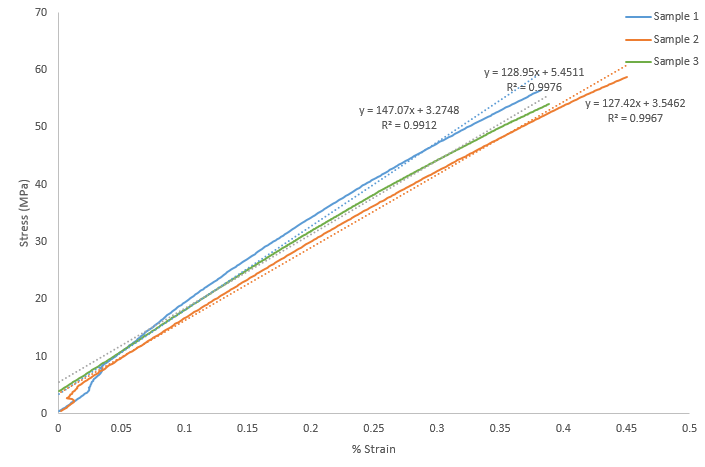
\includegraphics[width=.95\linewidth]{figures/PBT9_Tensile.png}
\caption{PBT9 Tensile Test}
\label{pbt9tensile}
\end{figure}

\begin{figure}[H]
\centering
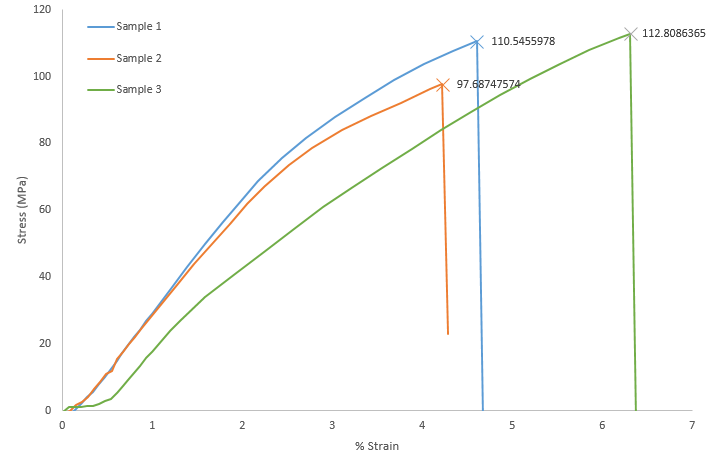
\includegraphics[width=.95\linewidth]{figures/PBT9_Fail.png}
\caption{PBT9 Test to Failure}
\label{pbt9fail}
\end{figure}

\begin{figure}[H]
\centering
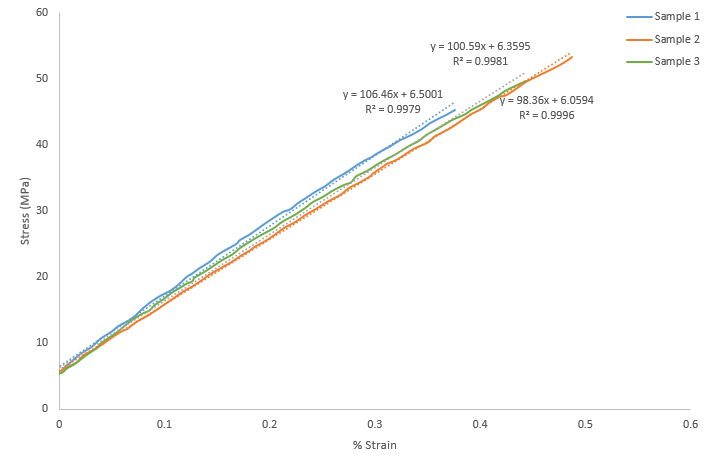
\includegraphics[width=.95\linewidth]{figures/PBT11_Tensile.png}
\caption{PBT11 Tensile Test}
\label{pbt11tensile}
\end{figure}

\begin{figure}[H]
\centering
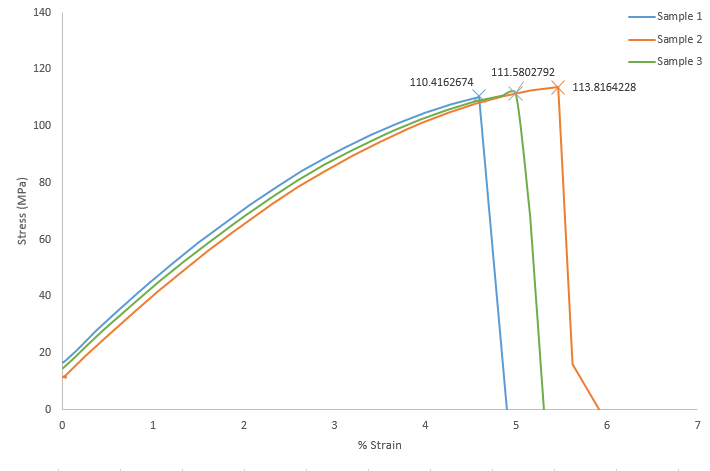
\includegraphics[width=.95\linewidth]{figures/PBT11_Fail.png}
\caption{PBT11 Test to Failure}
\label{pbt11fail}
\end{figure}

\begin{figure}[H]
\centering
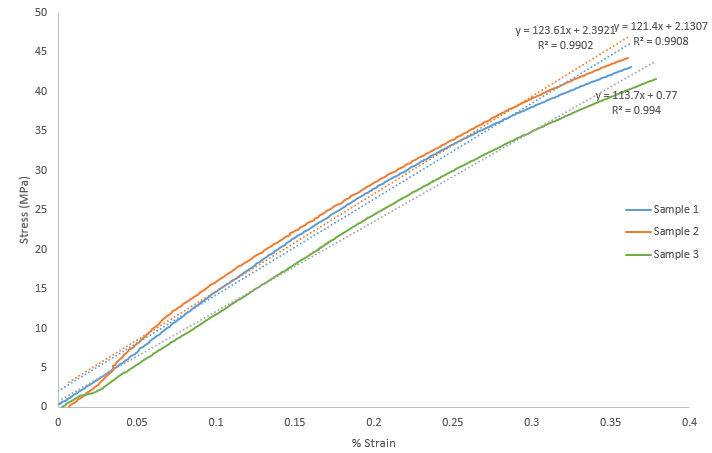
\includegraphics[width=.95\linewidth]{figures/PBT12_Tensile.png}
\caption{PBT12 Tensile Test}
\label{pbt12tensile}
\end{figure}

\begin{figure}[H]
\centering
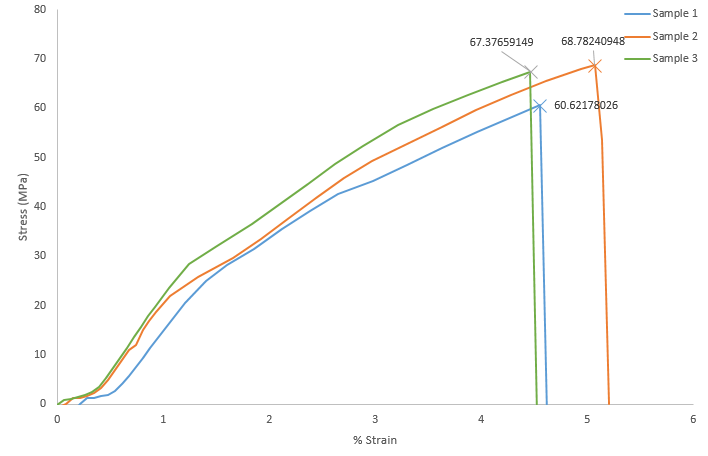
\includegraphics[width=.95\linewidth]{figures/PBT12_Fail.png}
\caption{PBT12 Test to Failure}
\label{pbt12fail}
\end{figure}

\begin{figure}[H]
\centering
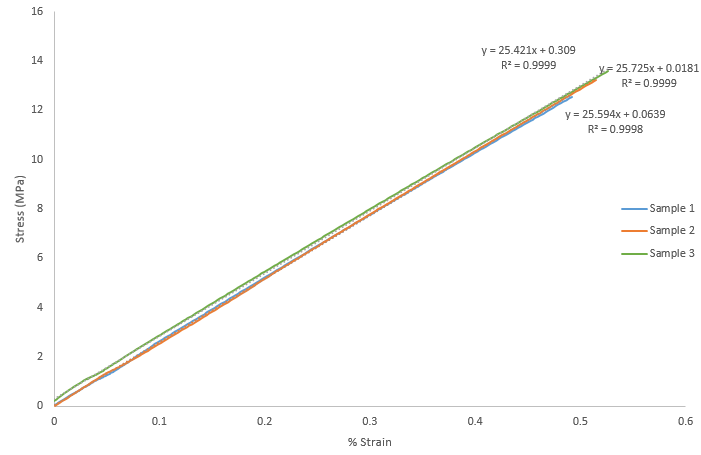
\includegraphics[width=.95\linewidth]{figures/PBT14_Tensile.png}
\caption{PBT14 Tensile Test}
\label{pbt14tensile}
\end{figure}

\begin{figure}[H]
\centering
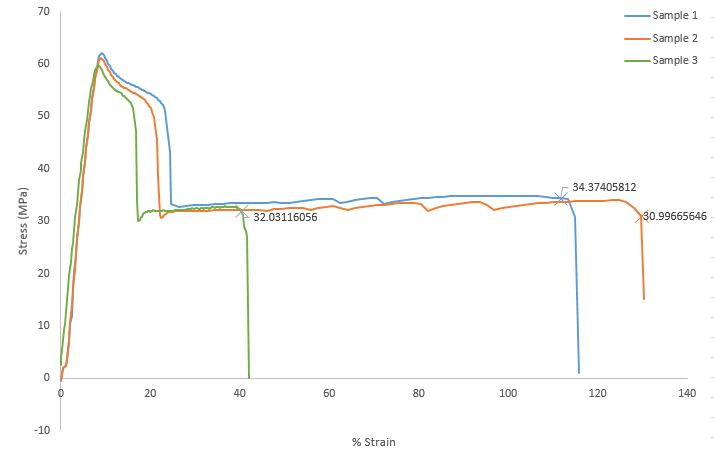
\includegraphics[width=.95\linewidth]{figures/PBT14_Fail.png}
\caption{PBT14 Test to Failure}
\label{pbt14fail}
\end{figure}

Observing these graphs, it is clear that the modulus is fairly consistent for each of the PBT samples, but when it comes to the fracture point, the test samples performed slightly differently. For PBT9, the fracture strength ranged from 97MPa up to 112MPa, with a strain at break of 4\% to 6\%. For PBT11, the data is more precise, with the fracture strength ranging from 110MPa to 113MPa, with a strain at break of 5\% to 6\%. For PBT12, the data is also fairly precise, with the fracture strength ranging from 60MPa to 67MPa, with a strain at break of 4.5\% to 5\%. Finally, PBT14 had precise fracture strengths (31MPa to 34MPa), but very diverse strains at break (40\% to 130\%).

Table \ref{tab:MaterialValues} shows the mechanical material properties of the fiber (E-Glass) and matrix (PBT) materials. These will be used later on when calculating the Young's Modulus and Fracture Stress of the samples. The Young's Modulus for PBT is determined from Figure \ref{pbt14tensile} and the fracture strength and yield stress for PBT is obtained from observing the yield points of Figure \ref{pbt14fail}.

\onehalfspacing
\begin{center}
\captionof{table}{Material Data for E-Glass Fiber and PBT Polymer} \label{tab:MaterialValues}
\begin{tabular}{p{2cm} || p{2.75cm} | p{2.75cm} | p{2.75cm} | p{2.75cm} }
\hline
\multicolumn{1}{c||}{Material} & Young's Modulus (MPa) & \(\sigma^*\), Fracture Strength (MPa) & Shear Modulus (MPa) & Yield Stress (MPa)\\
\hline
\hline
\(E-Glass\) & 70000 &  1750 & 881.6 & N/A \\
\(PBT\) & 2558 & 33.65 & N/A & 60.91\\
\hline
\end{tabular}
\end{center}
\singlespacing

\section{Discussion}

Using the values in Table \ref{tab:MeasuredValues} and Table \ref{tab:MaterialValues} the elastic modulus of the samples can be found using both the Halpin approach (Equation \ref{eq:halpin}) and simple equation (Equation \ref{eq:simple}). First, it is helpful to determine which set of equations are valid for this case. We assume for these calculations that the fibers are short, discontinuous and parallel to the load direction as seen through the pictures on the microscope. From this we can select the equations which are presented below. These equations require the \textit{critical fiber length}, \(\ell_c\), which is minimum length of fiber that is required to build up tensile stresses up in the fiber to the fracture strength. This is calculated using the following equation

\begin{equation}
\ell_c = \frac{\sigma^*_f r}{\tau^*_i}
\end{equation}
\\

The interfacial shear strength, \(\tau^*_i\), is found to be equal to the shear yield of the matrix, \(\tau^y_m\), which is determined by

\begin{equation}
\tau^*_i = \tau^y_m = 0.5 \sigma^y_m 
\end{equation}

The value for the yield strength for the matrix, as mentioned prior, can be found from \ref{tab:MaterialValues} to be 60.91 MPa.

\begin{equation} \label{eq:halpin}
\frac{E^{short}_{\downarrow \downarrow}}{E_m} = \frac{1+\xi \eta V_f}{1-\eta V_f}
\end{equation}

To calculate \(E_{\downarrow \downarrow}^{short}\) using the Halpin method, two variables are required, \(\eta\) and \(\xi\), which are calculated using the following:

\begin{equation}
\eta = \frac{E_f/E_m-1}{E_f/E_m+\xi}
\end{equation}

\begin{equation}
\xi = 2 \frac{l}{d} +40V^{10}_f
\end{equation}
\\
The values for the Young's Modulus of the fiber and the matrix can be found in Table \ref{tab:MaterialValues} and the ratio of  length, \(\ell\), over diameter, \textit{d} is the aspect ratio which is determined from the results of measuring the fibers and diameters from Table \ref{tab:MeasuredValues}.
\\
The simple method of calculating \(E_{\downarrow \downarrow}^{short}\) is shown in the following equation.

\begin{equation} \label{eq:simple}
E^{short}_{\downarrow \downarrow} = \eta_l E_f V_f + E_m(1-V_f)
\end{equation}

The simple method is developed from the rule of mixtures for a unidirectional lamina and applying a length correction factor, \(\eta_l\) which is found using the following equations.

\begin{equation}
\eta_l = 1- \left[\frac{\tanh 0.5\beta l}{0.5\beta l} \right]
\end{equation}

\begin{equation}
\beta=\left[\frac{2G_m}{E_fr^2 ln(\frac{R}{r})}\right]^{1/2}
\end{equation}
\\
The shear modulus for the matrix can be found in Table \ref{tab:MaterialValues}. The ratio of interfiber spacing, \textit{R} and fiber radius, \textit{r} can be found using the following equation from Hull \cite{hull}. This relationship is for hexagonally arranged fibers but because the ratio of \(\frac{R}{r}\) appearing in a logarithmic term in \(\beta\) , the hexagonal arrangement is acceptable to use as the result of the logarithmic term is sufficiently insensitive to fiber arrangement.

\begin{equation}
\frac{1}{V_f}=\left[\frac{R}{r}\right]^2
\end{equation}
\\

The \textit{critical fiber length} for the PBT samples are approximately 815 microns, and since the average fiber lengths found in the samples (Table \ref{tab:MeasuredValues}) are lower than the critical length, it is valid to use following equation for fractures stress of the composite. The values for the fiber and matrix fracture strength can be found in Table \ref{tab:MaterialValues}.
 
\begin{equation} \label{eq:fracture}
\sigma^*_{\downarrow \downarrow} = \left( \frac{l}{2l_c}\right) \sigma_f^* V_f + \sigma^*_m V_m
\end{equation}
\\

The results of these calculations are shown in the following table.

\onehalfspacing
\begin{center}
\captionof{table}{PBT9, PBT11, PBT12, and PBT14 Modulus and Fracture Stress} \label{tab:CalculatedValues}
\begin{tabular}{p{3.5cm} || p{2.cm} | p{2.cm} | p{2.cm} | p{2.cm}}
\hline
Sample & \multicolumn{1}{c|}{PBT9} & \multicolumn{1}{c|}{PBT11} & \multicolumn{1}{c|}{PBT12} & \multicolumn{1}{c}{PBT14} \\
\hline
\hline
\(E^{short}_{\downarrow \downarrow}\) Halpin (MPa)& 12658.3 &  10508.06 & 8376.91 & 2558\\
\(E^{short}_{\downarrow \downarrow}\) Simple (MPa)& 12256.6 & 10366.57 & 8338.3 & 2558\\
\(\sigma^*_{\downarrow \downarrow}\) (MPa)& 163.50 & 139.19 & 110.30 & 33.65\\
\(\ell_c (\mu m) \) & 815.28 & 814.93 & 815.64 & N/A\\
\hline
Halpin vs. Simple, \% Difference & 6.07 & 5.12 & 3.18 & 0\\
\hline
\end{tabular}
\end{center}
\singlespacing

Comparing the results of these tensile tests to the analytical Halpin data in Table \ref{tab:CalculatedValues}, it is clear that there is some degree of error between the experimental and analytical results for PBT11 and PBT12. It was previously when doing the experiment that the tensile test for PBT12 was done incorrectly, leading to erroneous values for determining the Young's Modulus.
\\
\bigskip
\onehalfspacing
\begin{center}
\captionof{table}{Tensile Test Data} \label{tab:ComparingValues}
\begin{tabular}{p{1.25cm} || p{1.5cm} | p{1.5cm} | p{1.5cm} | p{1.5cm} | p{1.5cm} | p{1.5cm} | p{1cm}}
\hline
 \multirow{2}{*}{Sample} & \multicolumn{3}{c|}{Young's Modulus (MPa)}  & 
   \multicolumn{3}{c|}{Fracture Stress (MPa)} & \multirow{2}{*}{\(V_f\)} \\
   & \multicolumn{1}{c}{Test} & \multicolumn{1}{c}{Calculated} & \multicolumn{1}{c|}{\% Error} & \multicolumn{1}{c}{Test} & \multicolumn{1}{c}{Calculated} & \multicolumn{1}{c|}{\% Error} &\\
\hline
PBT9 & 13448 & 12658.33 & 6.24 & 107.01 & 163.50 & 34.55 & 0.224\\
PBT11 & 10180.33 & 10508.06 & 3.12 & 111.94 & 139.19 & 19.58 & 0.179\\
PBT12 & 11957 & 8376.91 & 42.74 & 65.31 & 110.30 & 40.53 & 0.135 \\
PBT14 & 2558 & 2558 & 0 & 33.65 & 33.65 & 0 & 0\\
\hline
\end{tabular}
\end{center}
\singlespacing

Plotting the experimental and analytical values of the Young's Modulus and the Fracture Stress helps to exemplify the differences between the experimental and analytical results, as shown in Figures \ref{FScompare} and \ref{ModulusCompare}.

\begin{figure}[H]
\centering
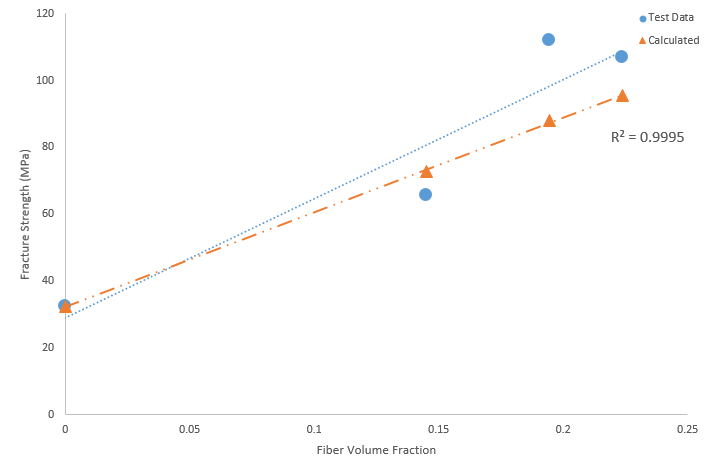
\includegraphics[width=.95\linewidth]{figures/fracture_stress_test_vs_calc.png}
\caption{Fracture Stress, Experimental vs. Analytical}
\label{FScompare}
\end{figure}

\begin{figure}[H]
\centering
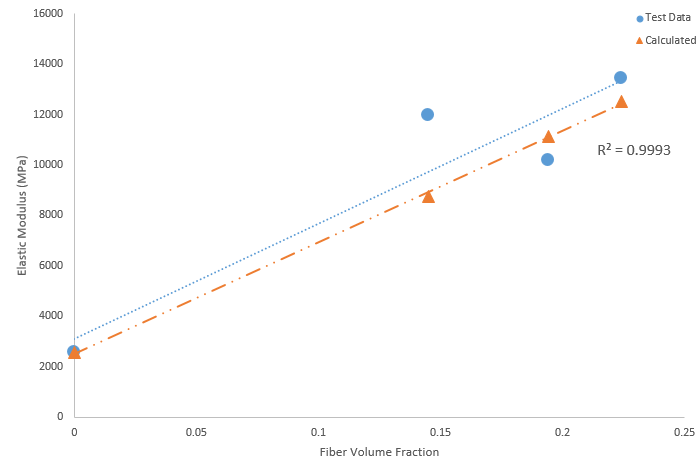
\includegraphics[width=.95\linewidth]{figures/modulus_test_vs_calc.png}
\caption{Young's Modulus, Experimental vs. Analytical}
\label{ModulusCompare}
\end{figure}

As mentioned before the test for PBT12 lead to erroneous results for the experimental Young's Modulus value. Therefore, PBT12 has the largest error of 42.74\%. The rest of the analytical values for PBT9 and PBT11 are within a 6\% error of the experimental values. It can be seen from Figure \ref{FScompare} that as you go from PBT14 which contains no fibers to PBT12, 11 and  9, the Young's Modulus increases. This is attributed to the increasing volume fraction of E-Glass fibers. This can be predicted from the relationship in Equation \ref{eq:simple} for the calculation of Young's Modulus using the simple, Rule of Mixtures (ROM) approach. The experimental values should also show the same trend as the analytical values, but again, because of the error with testing PBT12, it shows a higher Young's Modulus than that of PBT11 which is not to be expected. This trend is plotted in Figure \ref{FScompare}.
\singlespacing

When calculating the Young's Modulus, there is some discrepancy between the Halpin approach and the simple approach. Both approaches try to use the distribution and geometry of fibers to determine the overall Young's Modulus of the resulting composite. The ROM method utilises a correction factor, \(\eta_l\), based on the fiber packing geometry to estimate the microstructure of the composite while the Halpin approach uses the aspect ratio, \(\frac{\ell}{d}\). The calculated values for both as displayed in Table \ref{tab:CalculatedValues} show that the simple method has a slightly larger value than the Halpin method by up to a 6\% difference but have the same trend as shown in Figure \ref{ModulusCompare}.
\singlespacing

In terms of fracture strength the difference between the analytical and experimental values is up to 40\% higher which is a significant difference from the experimental value. This results in a steeper trend line for the analytical values for fracture strength. There is a discrepancy in the trend of the experimental data. As seen in fracture strength values in Figure \ref{FScompare}, the experimental data for PBT11 displays a higher fracture strength than that of PBT9. From the relationship given by Equation \ref{eq:fracture} and the trendline for the experimental values in Figure \ref{FScompare}, the trend should be linearly increasing fracture strength with increasing volume fraction of fiber.
\singlespacing

All these calculations do not take into account the presence of voids in the composite. The presence of voids in the composite affect the modulus since voids will effect the validity of the calculated volume fraction under the microscope. Voids also introduce stress concentrations during a tensile test of the composite which can cause the composite to fracture earlier than it should. This can be seen with the trend line in Figure \ref{FScompare} for the test data. PBT12 shows a lower fracture stress which may be attributed to the presence of much more voids than that of PBT11.
\singlespacing

Overall, in terms of the applicability of the composite rule of mixtures for comparison against experimental data, the rule of mixtures is an adequate way to estimate the Young's Modulus in the material but for fracture strength, it over-estimates the value by up to 40\% of the experimental value.

\section{Conclusion}


We did some stuff using some PBT samples for the sake of testing some stuff. From testing and analysis we learned that something about the PBT or composites and we got these results. From this we can say that blah blah blah or something. 

\newpage
\begin{thebibliography}{9}
\bibitem{manual}
R.A. Varin, \textit{"ME533 -- Composite Materials Laboratory Research Project}, 2017

\bibitem{hull} 
D. Hull, \textit{"An introduction to composite materials"}, Cambridge University Press, 1981

\end{thebibliography}
\end{document}